\documentclass[11pt,letterpaper]{article}
\usepackage[lmargin=1in,rmargin=1in,bmargin=1in,tmargin=1in]{geometry}
\usepackage{checkins}

\pgfplotsset{soldot/.style={color=black,only marks,mark=*},
		holdot/.style={color=black,fill=white,only marks,mark=*},
		compat=1.12
}

% -------------------
% Content
% -------------------
\begin{document}
\thispagestyle{title}

% 08/22
\checkin{08/22} If $\ds\lim_{x \to 5} f(x)= -3$, then $f(5)= -3$. \pspace

\sol The statement is \textit{false}. A function's limit (if it even exists) \textit{does not} have to be the same as the function's value at that limiting value---the function does not even have to be defined there! Consider the three examples below. \par
	\begin{center}
	% Left
	\fbox{%
	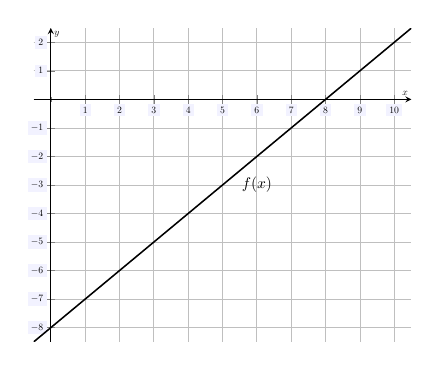
\begin{tikzpicture}[scale=0.7,every node/.style={scale=0.5}]
	\begin{axis}[
	grid=both,
	axis lines=middle,
	ticklabel style={fill=blue!5!white},
	xmin= -0.5, xmax=10.5,
	ymin= -8.5, ymax=2.5,
	xtick={-1,0,...,11},
	ytick={-8,-7,...,2},
	minor tick = {-9,-8,...,3},
	xlabel=\(x\),ylabel=\(y\),
	samples=20]
	\node at (6,-3) {\scalebox{1.6}{$f(x)$}};
	\addplot[thick, samples=5, domain= -0.5:10.5] {x - 8};
	\end{axis}
	\end{tikzpicture}
	} \hfill
	% Middle
	\fbox{%
	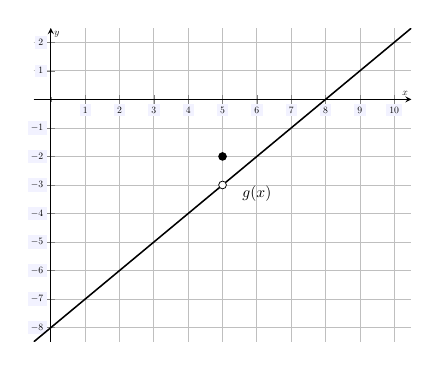
\begin{tikzpicture}[scale=0.7,every node/.style={scale=0.5}]
	\begin{axis}[
	grid=both,
	axis lines=middle,
	ticklabel style={fill=blue!5!white},
	xmin= -0.5, xmax=10.5,
	ymin= -8.5, ymax=2.5,
	xtick={-1,0,...,11},
	ytick={-8,-7,...,2},
	minor tick = {-9,-8,...,3},
	xlabel=\(x\),ylabel=\(y\),
	samples=20]
	\node at (6.0,-3.3) {\scalebox{1.6}{$g(x)$}};
	\addplot[thick, samples=5, domain= -0.5:10.5] {x - 8};
	\addplot[soldot] coordinates{(5,-2)};
	\addplot[holdot] coordinates{(5,-3)};
	\end{axis}
	\end{tikzpicture}
	} \hfill
	% Right
	\fbox{%
	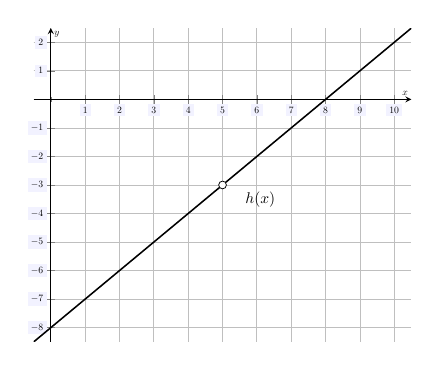
\begin{tikzpicture}[scale=0.7,every node/.style={scale=0.5}]
	\begin{axis}[
	grid=both,
	axis lines=middle,
	ticklabel style={fill=blue!5!white},
	xmin= -0.5, xmax=10.5,
	ymin= -8.5, ymax=2.5,
	xtick={-1,0,...,11},
	ytick={-8,-7,...,2},
	minor tick = {-9,-8,...,3},
	xlabel=\(x\),ylabel=\(y\),
	samples=20]
	\node at (6.1,-3.5) {\scalebox{1.6}{$h(x)$}};
	\addplot[thick, samples=5, domain= -0.5:10.5] {x - 8};
	\addplot[holdot] coordinates{(5,-3)};
	\end{axis}
	\end{tikzpicture}
	}
	\end{center} \par
For the graph of $f(x)$ on the left, $\ds\lim_{x \to 5} f(x)= -3$, so they are equal. However, observe that for $g(x)$ (the middle graph), we have $\ds\lim_{x \to 5} g(x)= -3$ but $g(5)= -2$, so that $\ds\lim_{x \to 5} g(x) \neq g(5)$. Similarly, in the graph of $h(x)$ on the right, $\ds\lim_{x \to 5} h(x)= -3$ but $h(-3)$ is not defined, so that $\ds\lim_{x \to 5} h(x) \neq h(-3)$. A function's value (if even defined) need not be related to its limit (if the limit even exists). \pvspace{1.3cm}



% 08/25
\checkin{08/25} The limit $\ds\lim_{x \to 0} \dfrac{\sin x}{x}= \text{DNE}$ because $\tfrac{\sin x}{x}$ becomes $\tfrac{0}{0}$ when one `plugs-in' $x= 0$ and $\frac{0}{0}$ is undefined. \pspace

\sol The statement is \textit{false}. In fact, $\ds\lim_{x \to 0} \dfrac{\sin x}{x}= 1$. Yes, $\tfrac{0}{0}$, $\pm\tfrac{\infty}{\infty}$, $0 \cdot \infty$, $\infty - \infty$, $0^0$, $1^\infty$, and $\infty^0$ are indeterminant/undefined expressions. However, that does not mean that the limit they arise from does not exist. The limit could exist or not---just like \textit{any} limit. `Running into' one of these expressions when evaluating a limit at its limiting value only means that one needs to try a different approach to determine if the limit exists or not. \pvspace{1.3cm}



% 08/27
\checkin{08/27} $\ds\lim_{x \to 0} \dfrac{\tan(5x)}{5x}= 1$ \pspace

\sol The statement is \textit{true}. Recall that $\ds\lim_{x \to 0} \dfrac{\sin(x)}{x}= 1$. We should think of this as $\ds\lim_{\Box \to 0} \dfrac{\sin \Box}{\Box}= 1$. But then\dots
	\[
	\lim_{x \to 0} \dfrac{\tan(5x)}{5x}= \lim_{x \to 0} \dfrac{\tfrac{\sin(5x)}{\cos(5x)}}{5x}= \lim_{x \to 0} \dfrac{\sin(5x)}{5x \cos x}= \lim_{x \to 0} \left( \dfrac{\sin(5x)}{5x} \cdot \dfrac{1}{\cos(5x)} \right)
	\]
Using the fact that $\ds\lim_{\Box \to 0} \dfrac{\sin \Box}{\Box}= 1$, we then have\dots
	\[
	\lim_{x \to 0} \dfrac{\tan(5x)}{5x}= \lim_{x \to 0} \left( \dfrac{\sin(5x)}{5x} \cdot \dfrac{1}{\cos(5x)} \right)= 1 \cdot \dfrac{1}{\cos(0)}= 1 \cdot \dfrac{1}{1}= 1
	\] \pvspace{1.3cm}



% 08/29
\checkin{08/29} $\ds\lim_{x \to 2^+} \dfrac{x - 3}{x - 2}= \infty$ \pspace

\sol The statement is \textit{false}. Observe that plugging-in $x= 2$, we obtain $\frac{-1}{0}$, which is undefined. However, this indicates that this is a `thinking limit'. Because in the limit, $x$ is `close' to 2, $x - 3$ is negative. As we approach 2 from the right, $x > 2$ so that $x - 2$ is positive. But then\dots
	\[
	\lim_{x \to 2^+} \dfrac{\overbrace{x - 3}^{-}}{\underbrace{x - 2}_{+}}= -\infty
	\] \pvspace{1.3cm}



% 09/03
\checkin{09/03} $\ds\lim_{x \to \infty} \dfrac{x^3 - 1}{1 - x^2}= -\infty$ \pspace

\sol The statement is \textit{true}. This is a rational limit. Observe that the degree of the numerator is 3 while the degree of the denominator is 2. Therefore, we know the limit will be $\pm\infty$. Observe that in the numerator, $x \to \infty$, so we know that $x^3 \to \infty$. In the denominator, we know that $x \to \infty$, so that $-x^2 \to -\infty$. Therefore, it should be that the limit tends to $-\infty$. We can confirm this intuition with the appropriate algebraic `trick': we divide the numerator and denominator by the `dominating' term in the denominator, which in this case is $x^2$:
	\[
	\lim_{x \to \infty} \dfrac{x^3 - 1}{1 - x^2}= \lim_{x \to \infty} \dfrac{x^3 - 1}{1 - x^2} \cdot \dfrac{1/x^2}{1/x^2}= \lim_{x \to \infty} \dfrac{\tfrac{x^3}{x^2} - \tfrac{1}{x^2}}{\tfrac{1}{x^2} - \tfrac{x^2}{x^2}}= \lim_{x \to \infty} \dfrac{x - \cancel{\tfrac{1}{x^2}}^{\,{}^0}}{\cancel{\tfrac{1}{x^2}}^{\,{}^0} - 1}= -\infty
	\] \pvspace{1.3cm}



% 09/05
\checkin{09/05} If $f(x)$ is a function and $\ds\lim_{x \to 1} f(x) = f(1)$, then $f(x)$ must be continuous at $x= 1$. \pspace

\sol The statement is \textit{true}. A function $f(x)$ is continuous at $x= a$ if $\ds f(a)= \lim_{x \to a} f(x)$. The statement of the problem states that $\ds\lim_{x \to 1} f(x)= f(1)$, i.e. $\ds f(1)= \lim_{x \to 1} f(x)$. Therefore, $f(x)$ is continuous at $x= 1$. Similarly, if we knew $f(x)$ was continuous at $x= 1$, then we would know that $\ds f(1)= \lim_{x \to 1} f(x)$. \pvspace{1.3cm}



% 09/07
\checkin{09/07} If $f(x)$ is given by\dots
	\[
	f(x)=
	\begin{cases}
	x + 1, & x \geq 0 \\
	4, & x < 0
	\end{cases}
	\]
Then $f(x)$ is differentiable at $x= 0$. \pspace

\sol The statement is \textit{false}. Recall that $f(x)$ is continuous at $x= a$ if $\ds f(a)= \lim_{x \to a} f(x)$ and that if a function is differentiable at $x= a$, then $f(x)$ is continuous at $x= a$. Therefore, $f(x)$ is continuous at $x= 0$ if and only if $\ds f(0)= \lim_{x \to 0} f(x)$. Observe that $f(0)= 0 + 1= 1$, $\ds\lim_{x \to 0^-} f(x)= \lim_{x \to 0^-} 4= 4$, and $\ds\lim_{x \to 0^+} f(x)= \lim_{x \to 0^+} (x + 1)= 0 + 1= 1$. Because $\ds\lim_{x \to 0^-} f(x) \neq \lim_{x \to 0^+} f(x)$, i.e. the left and right hand limits are not equal, $\ds\lim_{x \to 0} f(x)$ does not exist. But then $f(0) \neq \lim_{x \to 0} f(x)$, so that $f(x)$ is not continuous at $x= 0$. Because $f(x)$ is not continuous at $x= 0$, $f(x)$ cannot be differentiable at $x= 0$. \pspace

We can also verify this directly from the definition of the derivative. Recall that $\ds f'(a):= \lim_{h \to 0} \dfrac{f(a + h) - f(a)}{h}$. Here, we have $a= 0$ and $f(0)= 0 + 1= 1$. We compute this limit by computing the left and right hand limits. We have\dots
	\[
	\begin{aligned}
	\lim_{h \to 0^-} \dfrac{f(0 + h) - f(0)}{h}= \lim_{h \to 0^-} \dfrac{f(h) - f(0)}{h}= \lim_{h \to 0^-} \dfrac{4 - 1}{h}= \lim_{h \to 0^-} \dfrac{3}{h}= -\infty \\[0.3cm]
	\lim_{h \to 0^+} \dfrac{f(0 + h) - f(0)}{h}= \lim_{h \to 0^+} \dfrac{f(h) - f(0)}{h}= \lim_{h \to 0^+} \dfrac{(h + 1) - 1}{h}= \lim_{h \to 0^+} 1= 1 \\
	\end{aligned}
	\]
Because $\ds \lim_{h \to 0} \dfrac{f(0 + h) - f(0)}{h}$ does not exist, $f'(0)$ does not exist, i.e. $f(x)$ is not differentiable at $x= 0$. \pvspace{1.3cm}



% 09/10
\checkin{09/10} $\dfrac{d}{dx} \left( e^{\sin x} \right)= e^{\cos x}$ \pspace

\sol The statement is \textit{false}. Observe that the given solution, $e^{\cos x}$, has the derivative of both $e^x$ (which is $e^x$) and $\sin x$ (which is $\cos x$) simultaneously. However, all the derivative rules only ever have one taking the derivative of \textit{one} function at a time for any corresponding term. If we choose $f(x)= e^x$ and $g(x)= \sin x$, we have $f \big( g(x) \big)= f(\sin x)= e^{\sin x}$. We know that $f'(x)= e^x$ and $g'(x)= \cos x$. Using the chain rule, $\tfrac{d}{dx} f \big( g(x) \big)= f' \big( g(x) \big) \cdot g'(x)$, we have $\tfrac{d}{dx} e^{\sin x}= e^{\sin x} \cdot \cos x= e^{\sin x} \cos x$. Alternatively, using the `box method' or `onion approach', the first `layer' is $e^\Box{}$, whose derivative is $e^\Box{}$. We multiply by the derivative of the contents of $\Box{}$, which is the derivative of $\sin x$, i.e. $\cos x$. But then the derivative is $e^{\sin x} \cos x$. \pvspace{1.3cm}



% 09/11
\checkin{09/11} $\dfrac{d}{dx} \,\left( x^4 \csc(x) e^x \right)= 4x^3 \cdot \csc(x) e^x + -\csc x \cot x \cdot x^4 e^x + e^x \cdot x^4 \csc x$ \pspace

\sol The statement is \textit{true}. Although we can use the Product Rule: $\dfrac{d}{dx} (fg)= f'g + fg'$, it is simpler to recall that the Product Rule is a `one at a time rule.' That is, the product rule says to add together the product of the terms where the derivative of only one of the terms has been taken. Using this approach, we have\dots
	\[
	\begin{aligned}
	\dfrac{d}{dx} \,\left( x^4 \csc(x) e^x \right)&= \dfrac{d}{dx} (x^4) \cdot \csc x e^x + \dfrac{d}{dx} (\csc x) \cdot x^4 e^x + \dfrac{d}{dx}(e^x) \cdot x^4 \csc x \\[0.3cm]
	&= 4x^3 \cdot \csc(x) e^x + -\csc x \cot x \cdot x^4 e^x + e^x \cdot x^4 \csc x
	\end{aligned}
	\] \pvspace{1.3cm}



% 09/15
\checkin{09/15} $\dfrac{d}{dx} \left( \dfrac{x^2}{4x - 3} \right)= \dfrac{4(x^2) - 2x(4x - 3)}{(4x - 3)^2}$ \pspace

\sol The statement is \textit{false}. Recall that the quotient rule is given by $\frac{d}{dx} \left( \frac{f}{g} \right)= \frac{f' g - g' f}{g^2}$, i.e. the derivative of the bottom `gets the negative for its derivative' or the `\textbf{\underline{n}}umerator function' gets the \textbf{\underline{n}}egative. Observe that the given solution has the order of subtraction in the numerator reversed, i.e. it is the negative of the correct answer; that is, the numerator is `backwards' from the actual quotient rule. The correct answer should be:
	\[
	\dfrac{d}{dx} \left( \dfrac{x^2}{4x - 3} \right)= \dfrac{2x(4x - 3) - 4(x^2)}{(4x - 3)^2}
	\] \pvspace{1.3cm}



% 09/17
\checkin{09/17} If $f(x)$ is a function with $f(1)= 3$ and $f'(1)= 10$, then it should be that $f(0.8) \approx 1$. \pspace

\sol The statement is \textit{true}. The linearization of $f(x)$ at $x= a$ is $\ell_a(x)= f(a) + f'(a) \,\big( x - a \big)$. We know that if $x$ is `close' to $a$, then $f(x) \approx \ell_a(x)$. The linearization of the given $f(x)$ at $x= 1$ is $\ell_1(x)= f(1) + f'(1) \,\big( x - 1 \big)= 3 + 10(x - 1)$. But then we have\dots
	\[
	f(0.8) \approx \ell_1(0.8)= 3 + 10(0.8 - 1)= 3 + 10(-0.2)= 3 + (-2)= 1
	\] \pvspace{1.3cm}















\end{document}